% !TeX root = IAF2015-TouIST.tex
% la ligne précédente sert pour le logiciel TexWorks afin de pouvoir compiler ce fichier directement sans devoir ouvrir satoulouse_main.tex!

\nameTool\ est compos\'e de trois modules, mais l'utilisateur standard ne verra que l'un d'entre eux : l'interface. Dans la suite nous insistons principalement sur cette derni\`ere plut\^ot que sur le traducteur et le solveur.

Avec \nameTool\ on acc\`ede \`a un \'editeur puissant et convivial pour \'editer des formules logiques complexes et des contraintes vari\'ees comme :

$$\bigwedge_{i \in \{1..9\}} (P_i \IMPL Q_{i+1})$$

qui abr\`ege confortablement\\ 

$(P_1 \IMPL Q_2) \AND (P_2 \IMPL Q_3) \AND \ldots (P_9\IMPL Q_{10})$. 
\\

Une fois qu'un ensemble de formules a \'et\'e donn\'e \`a l'interface, sa satisfiabilit\'e peut \^etre v\'erifi\'ee : l'interface peut l'envoyer au prouveur qui retourne un mod\`ele s'il existe. Ensuite par l'interm\'ediaire de l'interface, l'utilisateur peut par exemple demander d'autres mod\`eles.


\section{D\'etail de ce qui peut \^etre fait avec \nameTool\label{sec:sat_tobedone}}

\subsection{Ensembles de domaines}
Avec le temps, nous avons remarqu\'e que nous avions souvent besoin d'\'ecrire des choses comme
$$\begin{aligned}\bigwedge_{i \in \{1..9\}} \bigwedge_{j \in \{1..9\}}\bigwedge_{ m\in \{A,B,C,D,E,F,G,H,I\}} \hspace{2cm}\\ \left( P_{i,j,m}\IMPL \bigwedge_{n \in \{A,B,C,D,E,F,G,H,I\}|m\neq n}\NOT P_{i,j,n}\right)\end{aligned}$$
Si on lit $P_{i,j,m}$ comme  ``il y a la lettre $m$ dans la case $(i,j)$'' d'une grille $9\times 9$, la formule ci-dessus exprime qu'il y a \emph{au plus} une lettre parmi `A' ... `I' dans chaque case. 

Ces ensembles $\{1..9\}$ et $\{A,B,C,D,E,F,G,H,I\}$ sont des \emph{ensembles de domaines}, avec \nameTool\ l'utilisateur peut d\'efinir autant d'ensembles de domaines qu'il le souhaite, par exemple :

\begin{verbatim}
begin sets
  set N=[1..9]
  set L=[A,B,C,D,E,F,G,H,I]
end sets
\end{verbatim}

et ainsi \'ecrire la formule ci-dessus comme
$$\bigwedge_{i \in N} \bigwedge_{j \in N}\bigwedge_{ m\in L}P_{i,j,m}\IMPL \bigwedge_{n \in L|m\neq n}\NOT P_{i,j,n}$$
De plus, les op\'erations usuelles sur les ensembles ($\cup$, $\cap$, $\setminus$, \ldots) peuvent \^etre utilis\'ees pour d\'efinir d'autres ensembles.


\subsection{Formules propositionelles}

Les formules de \nameTool\ sont bas\'ees sur des variables propositionnelles (qui peuvent \^etre indic\'ees) et les op\'erateurs logiques usuels ($\AND$, $\OR$, $\IMPL$, $\NOT$, $\IFF$). Ainsi on peut taper des formules usuelles simples comme $Pluie \IMPL Nuages$. Mais en plus, nous fournissons des op\'erateurs logiques de haut niveau qui permettent d'exprimer des assertions complexes dans une forme tr\`es compacte.

\subsubsection*{Conjonctions et disjonctions g\'en\'eralis\'ees}
Elles permettent d'exprimer des conjonctions et des disjonctions sur des formules contenant des param\`etres qui varient, par exemple :
\begin{itemize}
\item $ \bigwedge_{i \in N} P_i$, o\`u $N$ est l'ensemble de domaine d\'efini pr\'ec\'edemment.\\
  Elle repr\'esente la conjonction
  $P_1 \AND P_2 \AND \ldots \AND P_9$. 
\item $\bigvee_{i \in E} P_i$.
\end{itemize}

Bien s\^ur, ces op\'erateurs peuvent \^etre imbriqu\'es avec presque aucune limite, comme dans
$$\bigwedge_{i \in N} \bigwedge_{j \in N}\bigvee_{ m\in L}P_{i,j,m}$$

indiquant que dans chaque cellule se trouve au moins une lettre.


\subsubsection*{Contraintes de cardinalit\'e}
C'\'etait l'un des sujets ``laiss\'e pour le futur" de \cite{GaScSt2011}.
Ces op\'erateurs logiques moins classiques sont disponibles dans \nameTool\ : il permettent de r\'eduire drastiquement la taille de certaines formules, ce sont : $\atM{}{}$, $\atL{}{}$ et $\exact{}{}$.\\ L'exemple suivant d\'ecrit leur signification :
\begin{itemize}
\item $\atM{i \in N}{2} P_i$ repr\'esente ``pour au plus deux valeurs de $i \in N$ $P(i)$ est vraie;
\item $\atL{i \in N}{2} P_i$ repr\'esente ``pour au moins deux valeurs de $i \in N$ $P(i)$ est vraie;
\item $\exact{i \in N}{2} P_i$ repr\'esente ``pour exactement deux valeurs de $i \in N$ $P(i)$ est vraie.
\end{itemize}
La disjonction g\'en\'eralis\'ee est en fait un cas particulier de ceci : au moins une est vraie, la conjonction aussi : au plus 0 est fausse, et le ou exclusif peut \^etre vu comme : exactement une parmi deux est vraie. \\
Rappelons qu'avec des op\'erateurs logiques classiques et avec $N$ contenant 9 elements, $\atM{i \in N}{3} P_i$ devrait n\'ecessiter une formule contenant 84 propositions $P_i$ puisque cela revient \`a choisir 3 parmi 9 ce qui donne $\binom{9}{3}$ possibilit\'es, et ni $\bigwedge$ ni $\bigvee$ n'aideraient beaucoup. 

\subsubsection*{Contraintes et calculs sur des index}

Souvent nous avons besoin d'ajouter des contraintes sur les index, par exemple :
$$\bigwedge_{i \in E } \bigwedge_{j \in E  | i \neq j}P_{i,j}$$
qui signifie que $P_{i,j}$ est vraie lorsque $i\neq j$. 

C'\'etait la seule contrainte disponible dans \satoulouse, maintenant dans \nameTool\ la gamme de possibilit\'es \`a \'et\'e largement enrichie. Les contraintes peuvent inclure des op\'erateurs usuels de comparaison comme $<$, $>$, $\leq$, $\geq$, $\neq$, $=$ et ces comparaisons peuvent s'appliquer non seulement aux indices, mais aussi \`a toute expression arithm\'etique impliquant des index et $+$, $-$, $*$, $/$, $\mod$, $\sqrt{\phantom{x}}$. 

Exprimer une phrase comme ``chaque case $(i,j)$ contient un nombre qui n'est pas \'egal \`a $i+j$'' donnera :
$$\bigwedge_{i \in N } \bigwedge_{j \in N} \bigvee_{k \in N|k\neq i+j} P_{i,j,k}$$
Bien s\^ur, \emph{toutes ces phrases} pourraient \^etre exprim\'ees avec les op\'erateurs logiques usuels bruts, mais ceci serait un travail fastidieux. N\'eanmoins, les \'etudiants doivent savoir ce qui est derri\`ere la sc\`ene, et qu'une telle formule est l'abr\'eviation de quelque chose comme :
$$P_{1,1,1}\vee P_{1,1,3}\vee P_{1,1,4}\ldots P_{1,2,1}\vee P_{1,2,2}\vee P_{1,2,4}\vee \ldots $$
qui est tr\`es long et terne.



\subsection{Aspects techniques}

\subsubsection*{Langage d'entr\'ee vs Langage d'affichage}

Les formules que nous avons vues pr\'ec\'edemment sont \'ecrites dans le \emph{langage d'affichage} (style \LaTeX), mais tous ces symboles ne sont pas disponibles sur les claviers, ainsi pour \'ecrire les formules et ensembles de domaines, l'utilisateur utilisera le \emph{langage d'entr\'ee}.
Par exemple, la formule pr\'ec\'edente et l'ensemble associ\'e $N$ seront tap\'es :
\begin{verbatim}
begin sets
  set N=[1..9]
  set L=[A,B,C,D,E,F,G,H,I]
end sets

begin formula
  bigand i in N:
    bigand j in N:
      bigor k in N when k <> i+j:
        P(i,j,k)
...
end formula
\end{verbatim}
Mais \nameTool\ les affiche imm\'ediatement en style \LaTeX. 
En outre, les formules peuvent \^etre tap\'ees \`a la main dans la fen\^etre d'\'edition, ou introduites dans une sorte d'\'editeur dirig\'e par la syntaxe, en raffinant progressivement l'arbre syntaxique, ou encore elles peuvent \^etre import\'ees \`a partir d'un fichier externe.




\begin{figure}[ht]
  \centering
  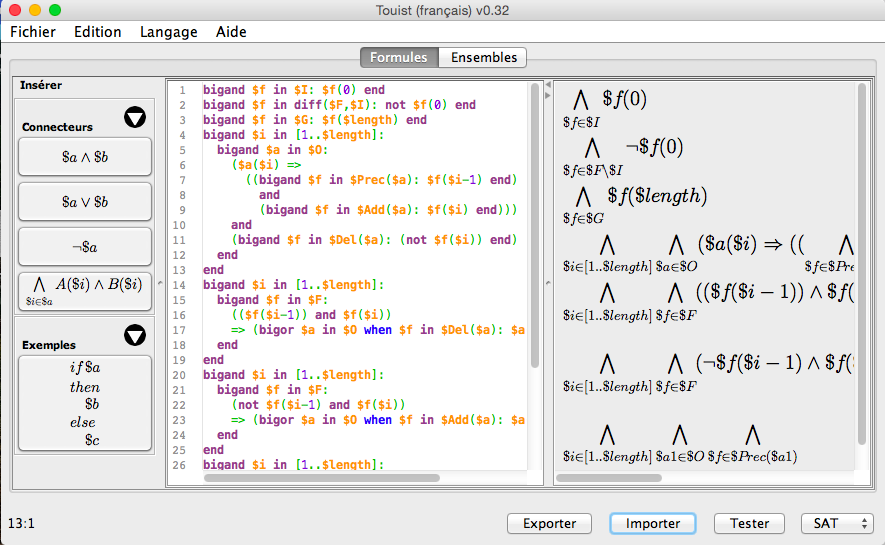
\includegraphics[scale=.26]{touist1.png}
  \caption{Interface de TouIST}
  \label{fig:touist}
\end{figure}

%\subsection{Be familiar with the notion of satisfiability}
%
%During our course, we give to the students easy exercises of formalization like:
%
%``A robbery happened last night. Inspector Lestrade is on the premises. The
%thief has been seen: he is small  and he left footprints of size
%40\footnote{French size... }. There are three suspects: A, B or C. A is tall
%and takes size 43 shoes. B is small and takes size 40 shoes. C is small and
%takes size 43 shoes. Who is the thief?'' (NB: they will have to elicit the
%fact that no one who takes size 43 wears 40). 
%
%\nameTool{} is used to enter such formalization into the computer and solve this kind of problems in order to accustom students with it, but such examples can still be treated by hand. Hence, we consider far bigger problems.
%
%But of course, in order to correctly interpret the results, i.e.\ satisfiable or unsatisfiable, they need to know what these words mean, and what information can be extracted from the solution the prover finds. 

%\subsection{Logic programming}
%
%Let's take a look at an example, the coding of a particularly simple form of
%Sudoku (9$\times$9 cells) for the sake of clarity. Remember that in a
%Sudoku, the player is requested to fill in an $9 \times 9$ grid with numbers
%ranging from 1 to $9$, such that some conditions are satisfied. To express the
%fact that at position $(i,j)$ on the grid, there is a unique number $9$, we
%use a number of constraints, for example (see screenshot):
%\begin{itemize}
%\item The domain of values is $E=\{1,\dots, 9 \}$
%\item In each cell at position $i,j$ there is at least one $n \in E$
%\item Each cell $(i,j)$  contains at most one $n\in N$
%\item Each line and column contains each $n$ of $ E$  exactly once
%\item There are nine regions which must contain each $n$ of $ E$  exactly once
%\item The game starts with already filled cells, this initial setting being described by a conjunction like $p_{1, 2, 3} \land p_{1, 6, 1} \land p_{2, 3, 6} \wedge \dots$ (there is 3 in cell (1, 2), there is 1 in cell (1, 6), there is 6 in cell (2, 3), etc.)
%\end{itemize}


%
%\begin{figure}[ht]
%  \centering
%  \includegraphics[width=\textwidth]{Figures/valuation.png}
%  \caption{Example of a valuation returned for the Sudoku problem of Figure~\ref{fig:satoulouse}}
%  \label{figure:valuation}
%\end{figure}


%%% Local Variables:
%%% mode: latex
%%% TeX-master: "satoulouse_main"
%%% End:
